\documentclass{beamer}
%\usepackage{beamerarticle}
\usepackage{pgf} 
\usepackage{heppennames}
\usepackage{hepnicenames}
\usepackage{graphicx} 
\usepackage{multirow}
\usepackage{amsbsy,amsmath,amssymb}


\usepackage{CJK}

\mode<presentation>
{
\usetheme{Singapore}
  \setbeamercovered{transparent}
   \setbeamertemplate{footline}[frame number] 
  \setbeamertemplate{navigation symbols}{ 
  \insertslidenavigationsymbol
  \insertframenavigationsymbol
  \insertsubsectionnavigationsymbol
  \insertsectionnavigationsymbol
  \insertdocnavigationsymbol
  \insertbackfindforwardnavigationsymbol
  \hskip 0.3cm
  %\insertframenumber / \inserttotalframenumber  % <<< frame #
  %\insertpagenumber / \insertpresentationendpage % <<< page #
} 
}

\usepackage[english]{babel}
\usepackage[latin1]{inputenc}

% font definitions, try \usepackage{ae} instead of the following
% three lines if you don't like this look
\usepackage{mathptmx}
\usepackage[scaled=.90]{helvet}
\usepackage{courier}


\usepackage[T1]{fontenc}

\title{Presentation}

%\subtitle{}

% - Use the \inst{?} command only if the authors have different
%   affiliation.
%\author{F.~Author\inst{1} \and S.~Another\inst{2}}
\author{St\'ephane Poss}
\institute[CERN]
{
Job reference: INPS12-8
}

% - Use the \inst command only if there are several affiliations.
% - Keep it simple, no one is interested in your street address.


\date{\today}


% This is only inserted into the PDF information catalog. Can be left
% out.
\subject{ILCDIRAC}



% If you have a file called "university-logo-filename.xxx", where xxx
% is a graphic format that can be processed by latex or pdflatex,
% resp., then you can add a logo as follows:

% \pgfdeclareimage[height=0.5cm]{university-logo}{university-logo-filename}
% \logo{\pgfuseimage{university-logo}}



% Delete this, if you do not want the table of contents to pop up at
% the beginning of each subsection:
\AtBeginSubsection[]
{
\begin{frame}<beamer>
\frametitle{Outline}
\tableofcontents[currentsection,currentsubsection]
\end{frame}
}

% If you wish to uncover everything in a step-wise fashion, uncomment
% the following command:

%\beamerdefaultoverlayspecification{<+->}
\begin{document}

\begin{frame}
\titlepage
\end{frame}

\begin{frame}
\frametitle{Curriculum}
\begin{enumerate}
  \item 2001-2004, Physics Bachelor \\
    {\scriptsize (Universit\'e de la M\'editerrann\'ee, Marseille, France)}
  \item 2004-2006, Physics Master \\
    {\scriptsize(Universit\'e de la M\'editerrann\'ee, Marseille, France)}
  \item 2006-2009, PhD. Flavour tagging in LHCb \\
    {\scriptsize(Universit\'e de la M\'editerrann\'ee, Marseille, France)}
  \item 2010-now, CERN fellowship
\end{enumerate}
\end{frame}
 
%\part{Initial interest in High Energy Physics}
%\begin{frame}
%\partpage
%\end{frame}
% \begin{frame}
% \frametitle{Initial interest in High Energy Physics}
% First interest in HEP: at {\color{blue}15 years old}, high school:
% \begin{columns}
% \begin{column}[T]{3.5cm}
% \begin{center}
% 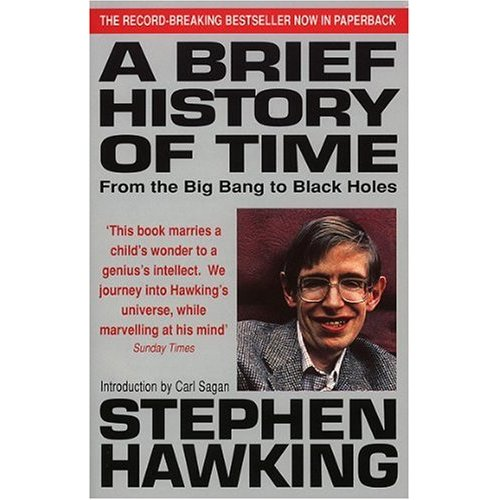
\includegraphics[width=4cm]{briefhist}
% \end{center}
% \end{column}
% \begin{column}[T]{3cm}
% \begin{center}
% 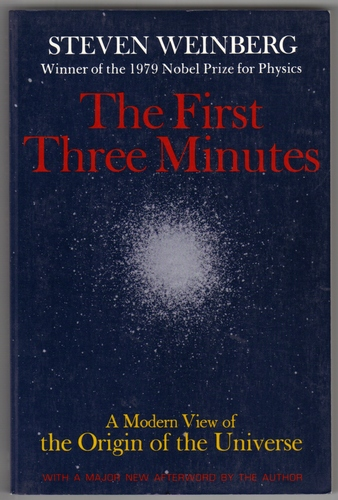
\includegraphics[width=2.7cm]{firstthree}
% \end{center}
% \end{column}
% \begin{column}[T]{5cm}
% \begin{center}
% 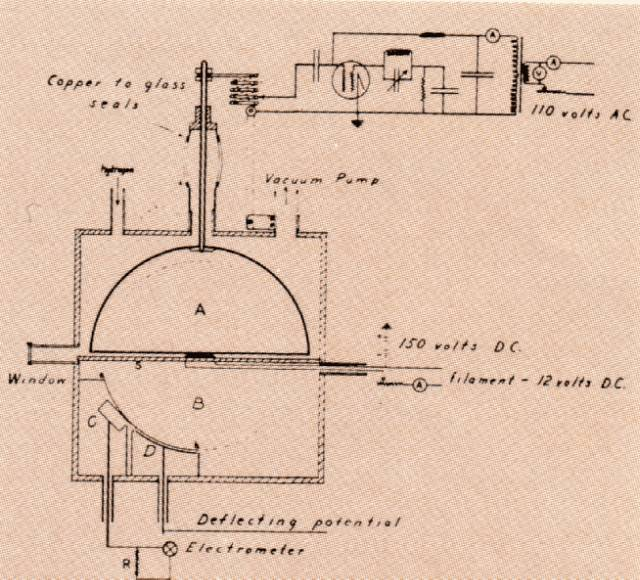
\includegraphics[width=4.5cm]{firstcyclo}
% \end{center}
% \end{column}
% \end{columns}
% ~\\
% Wanted to work on accelerator physics, and make new discoveries\ldots\\
% \begin{center} 
% \alert{Decided to study high energy physics!}
% \end{center}
% \end{frame}
% 
% \begin{frame}
% \frametitle{Initial interest (Cont'd)}
% {\color{blue}Amazed by the cyclotron} studied in school:
% \begin{center}
% 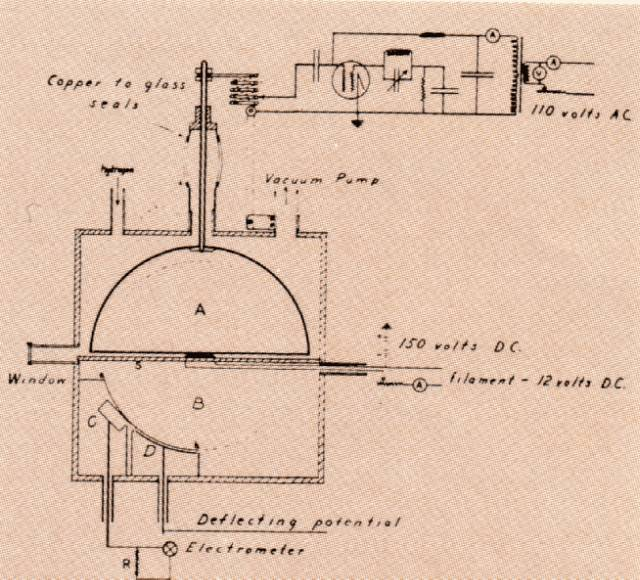
\includegraphics[width=6cm]{firstcyclo}
% \end{center}
% Wanted to work on accelerator physics, and make new discoveries\ldots\\
% \begin{center} 
% \alert{Decided to study high energy physics!}
% \end{center}
% \end{frame}

% \begin{frame}
% \frametitle{Initial interest (Cont'd)}
% University curriculum:
% \begin{itemize}
%   \item First 2 years in Aix-en-Provence, 
%   \item Then had to {\color{blue} move to Marseille} for the rest: Universit\'e
%   de la M\'editerrann\'ee
%   \item {\color{blue} Discovered CPPM} during first trip to University
%   \begin{center}
%   
\includegraphics[width=2cm]{logocppm}
%   \end{center}
%   \item Knew I would do my \alert{PhD. thesis there} \pause
%   \item Managed to do that
% \end{itemize}
% \end{frame}
{
\usebackgroundtemplate{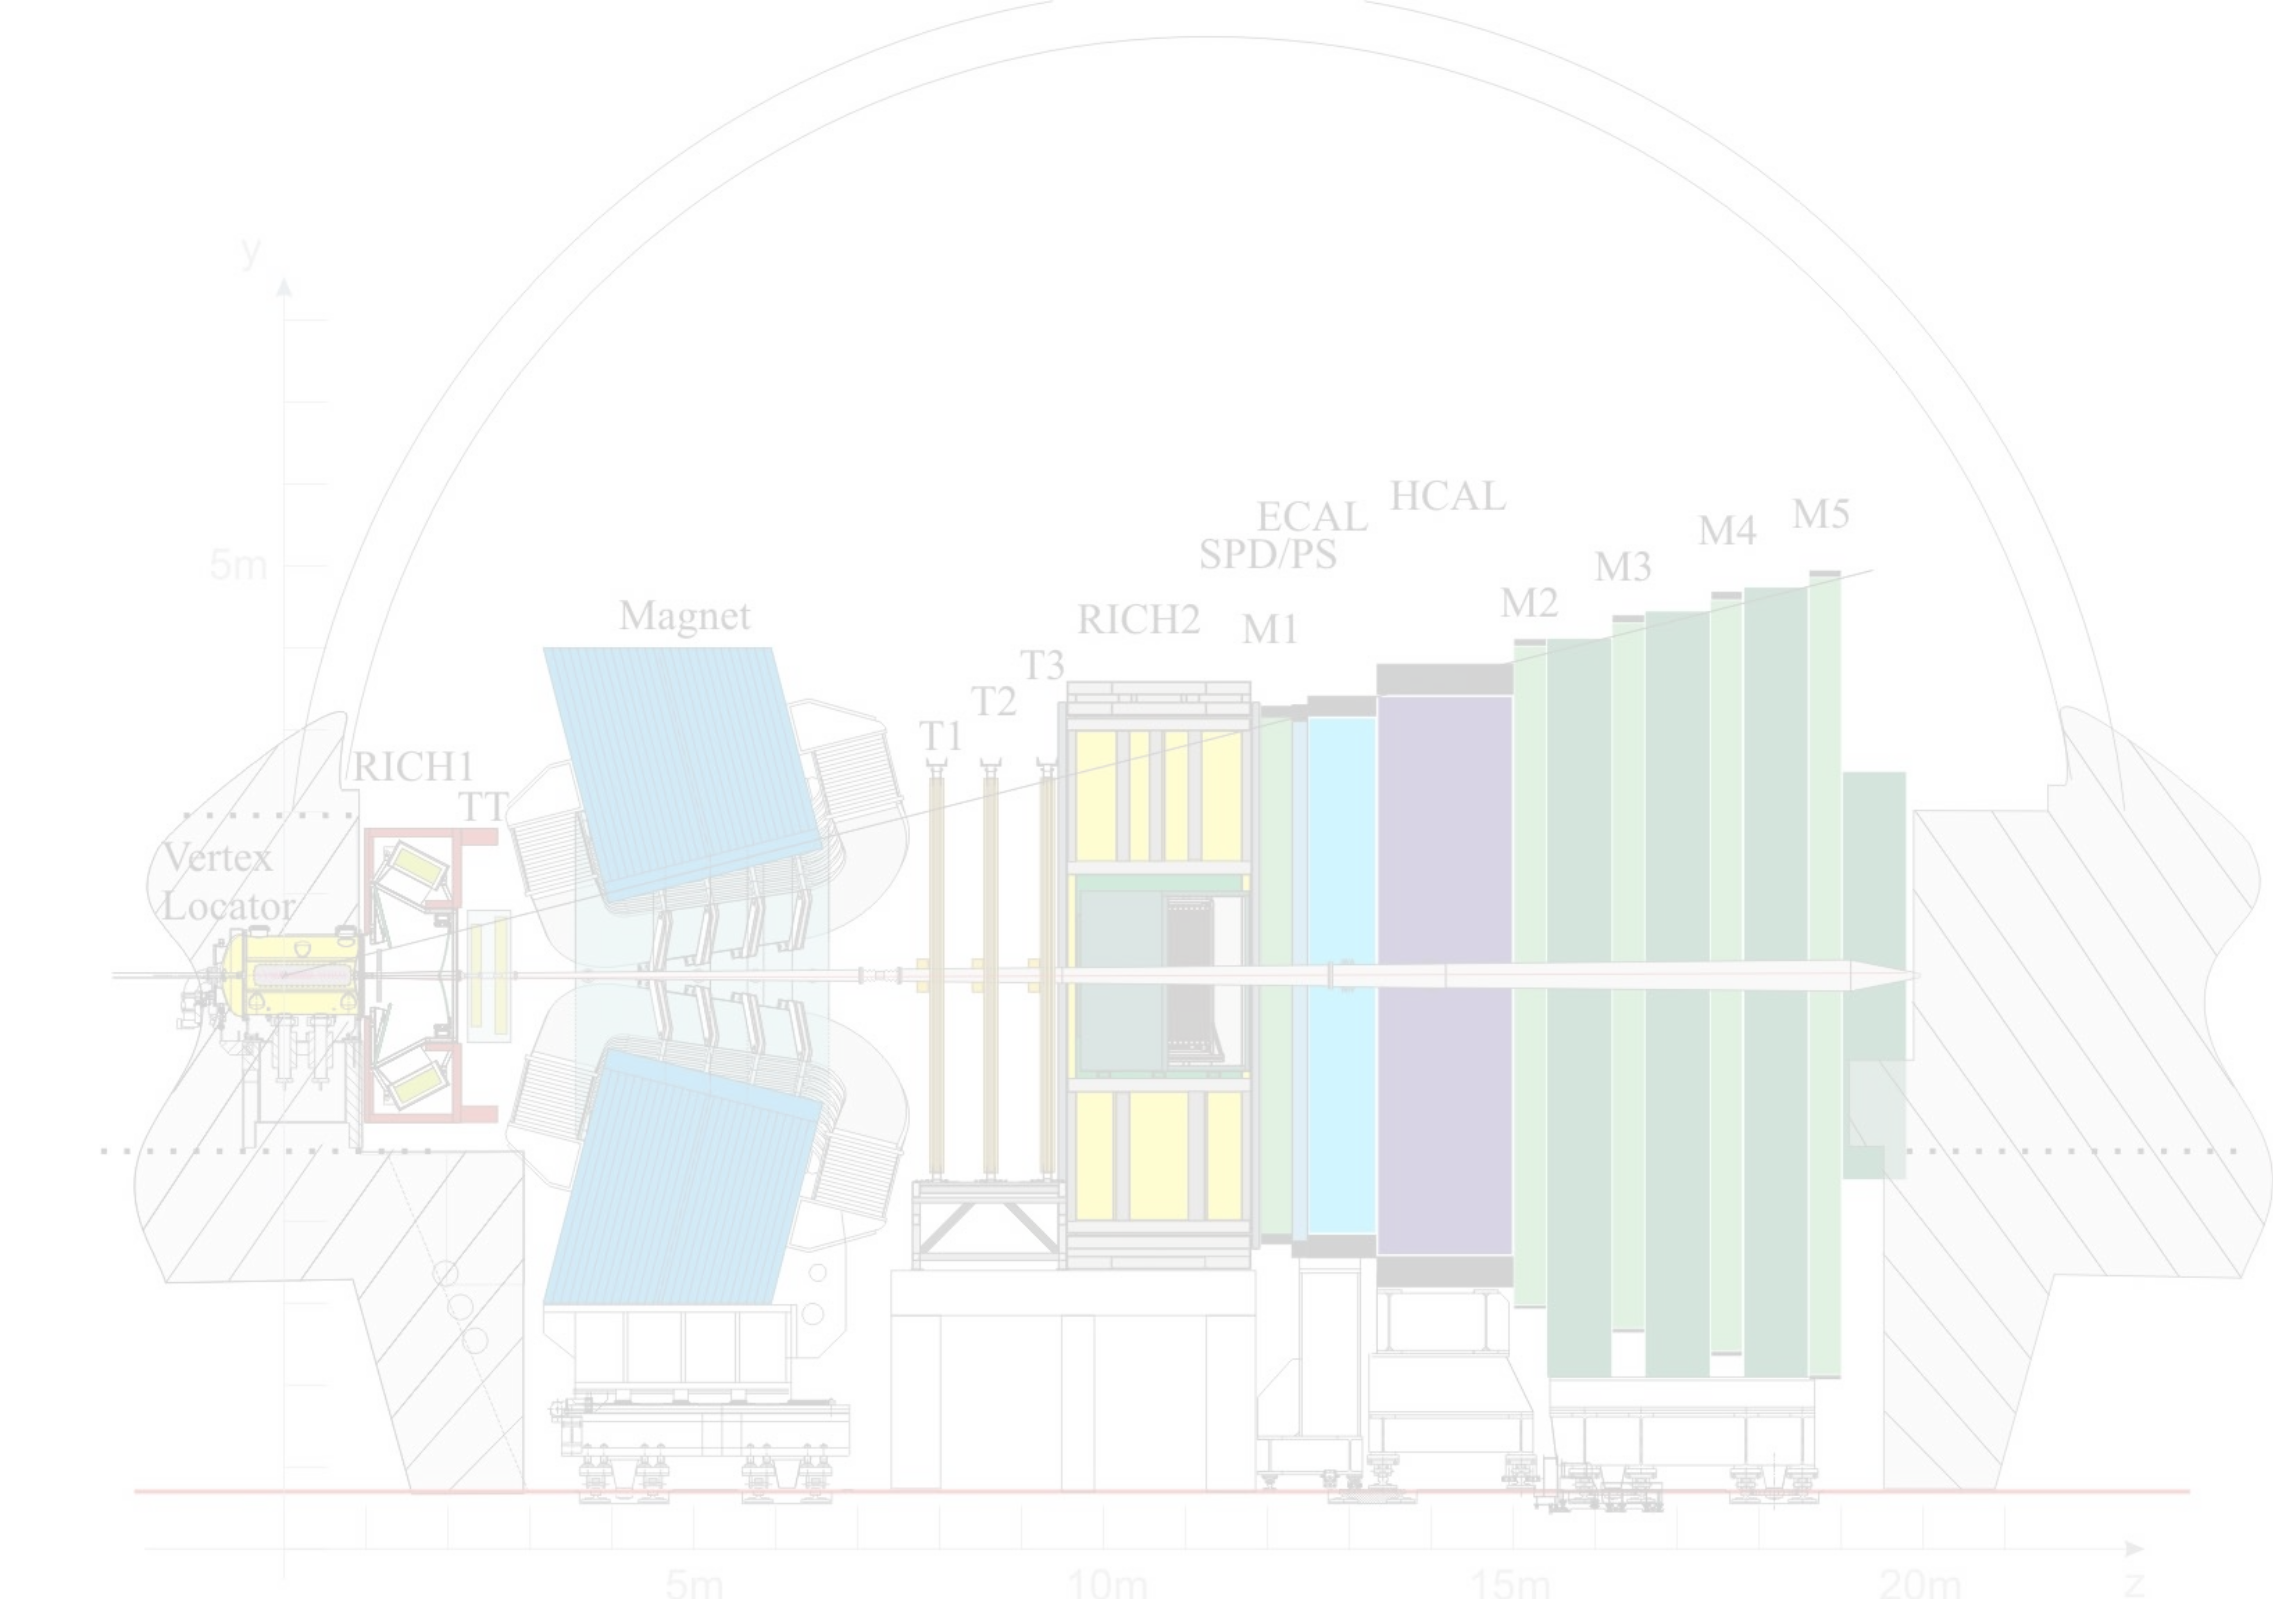
\includegraphics[width=\paperwidth]{gene-2008-002_01_t1}}

\part{2006-2009, PhD.: Flavour tagging in LHCb} 
\begin{frame}
\partpage
\end{frame}
\begin{frame}
\frametitle{Flavour tagging in LHCb}
Definition: determine the flavour (charge) of a b quark at its production.
\begin{center}
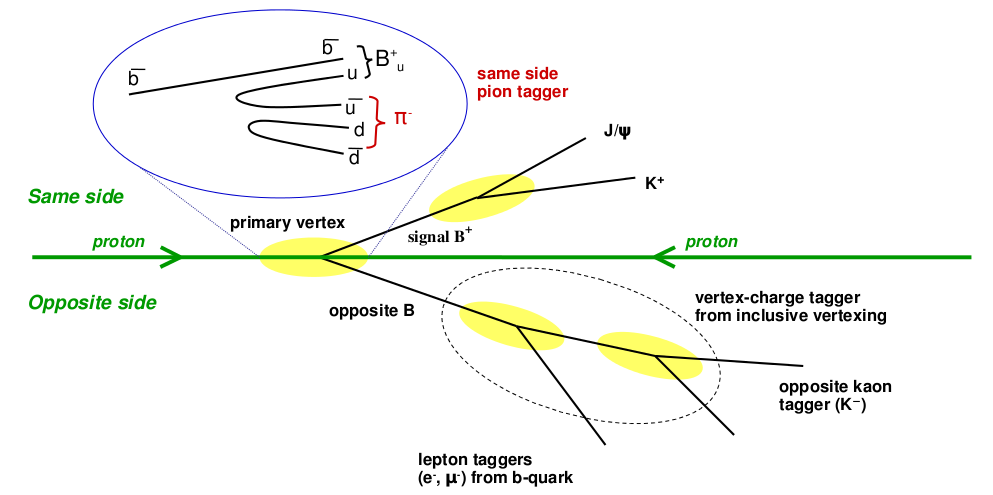
\includegraphics[width=11cm]{tagging.png}
\end{center}
Essential for many \alert{CP violation measurements}: $\sin(2\phi_1)$, $\beta_s$,
etc.
\end{frame}
}
% {
% \usebackgroundtemplate{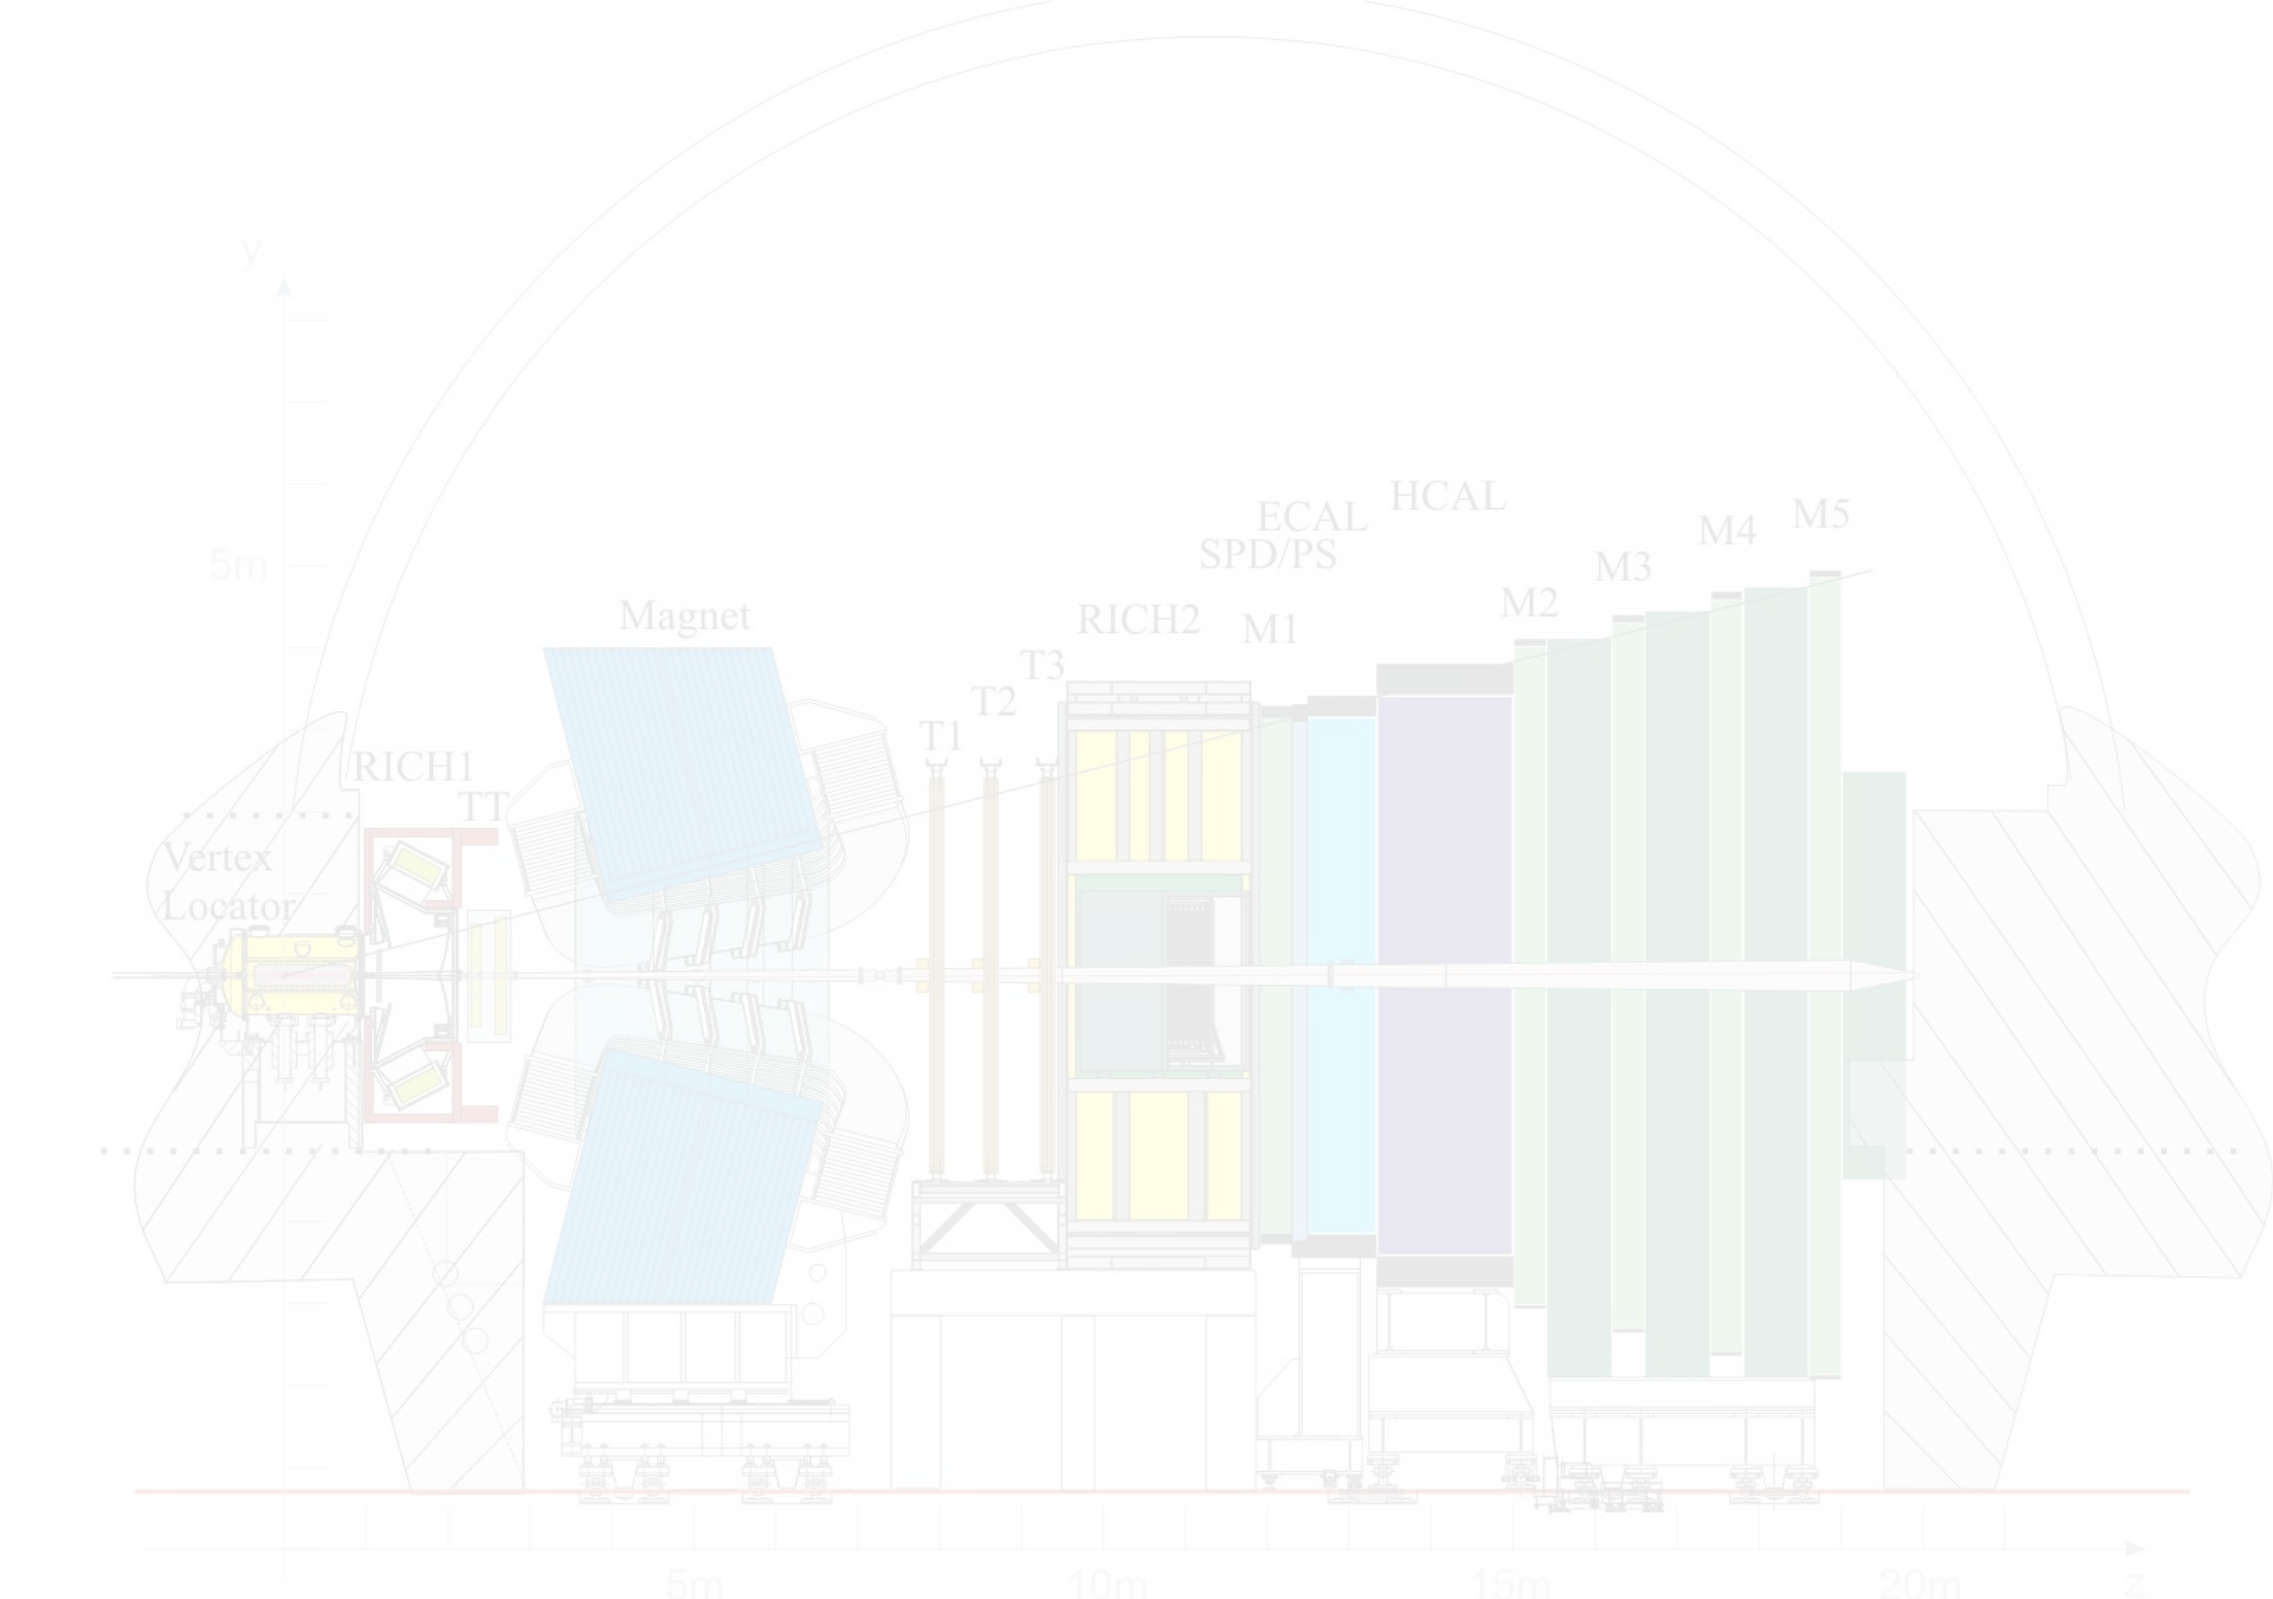
\includegraphics[width=\paperwidth]{gene-2008-002_01_t2}}

% \begin{frame}
% \frametitle{From interships to the PhD.}
% \begin{itemize}
%   \item Started studying \alert{flavour tagging} between Bachelor and Master,
%   in the {\color{blue} LHCb group at CPPM, Marseille, Fr.}\\
%   ~\\
%   \item Internship at \alert{CERN in summer 2005}: Flavour tagging in
%     LHCb's event display, Panoramix\\
%   ~\\
%   \item Master's {\color{blue} internship}: Study of secondary
%   vertex reconstruction for flavour fagging in LHCb\\
%   ~\\
%   \item \alert{Accepted as PhD. student} in the LHCb group of CPPM
% \end{itemize}
% \end{frame}
% }
{
\usebackgroundtemplate{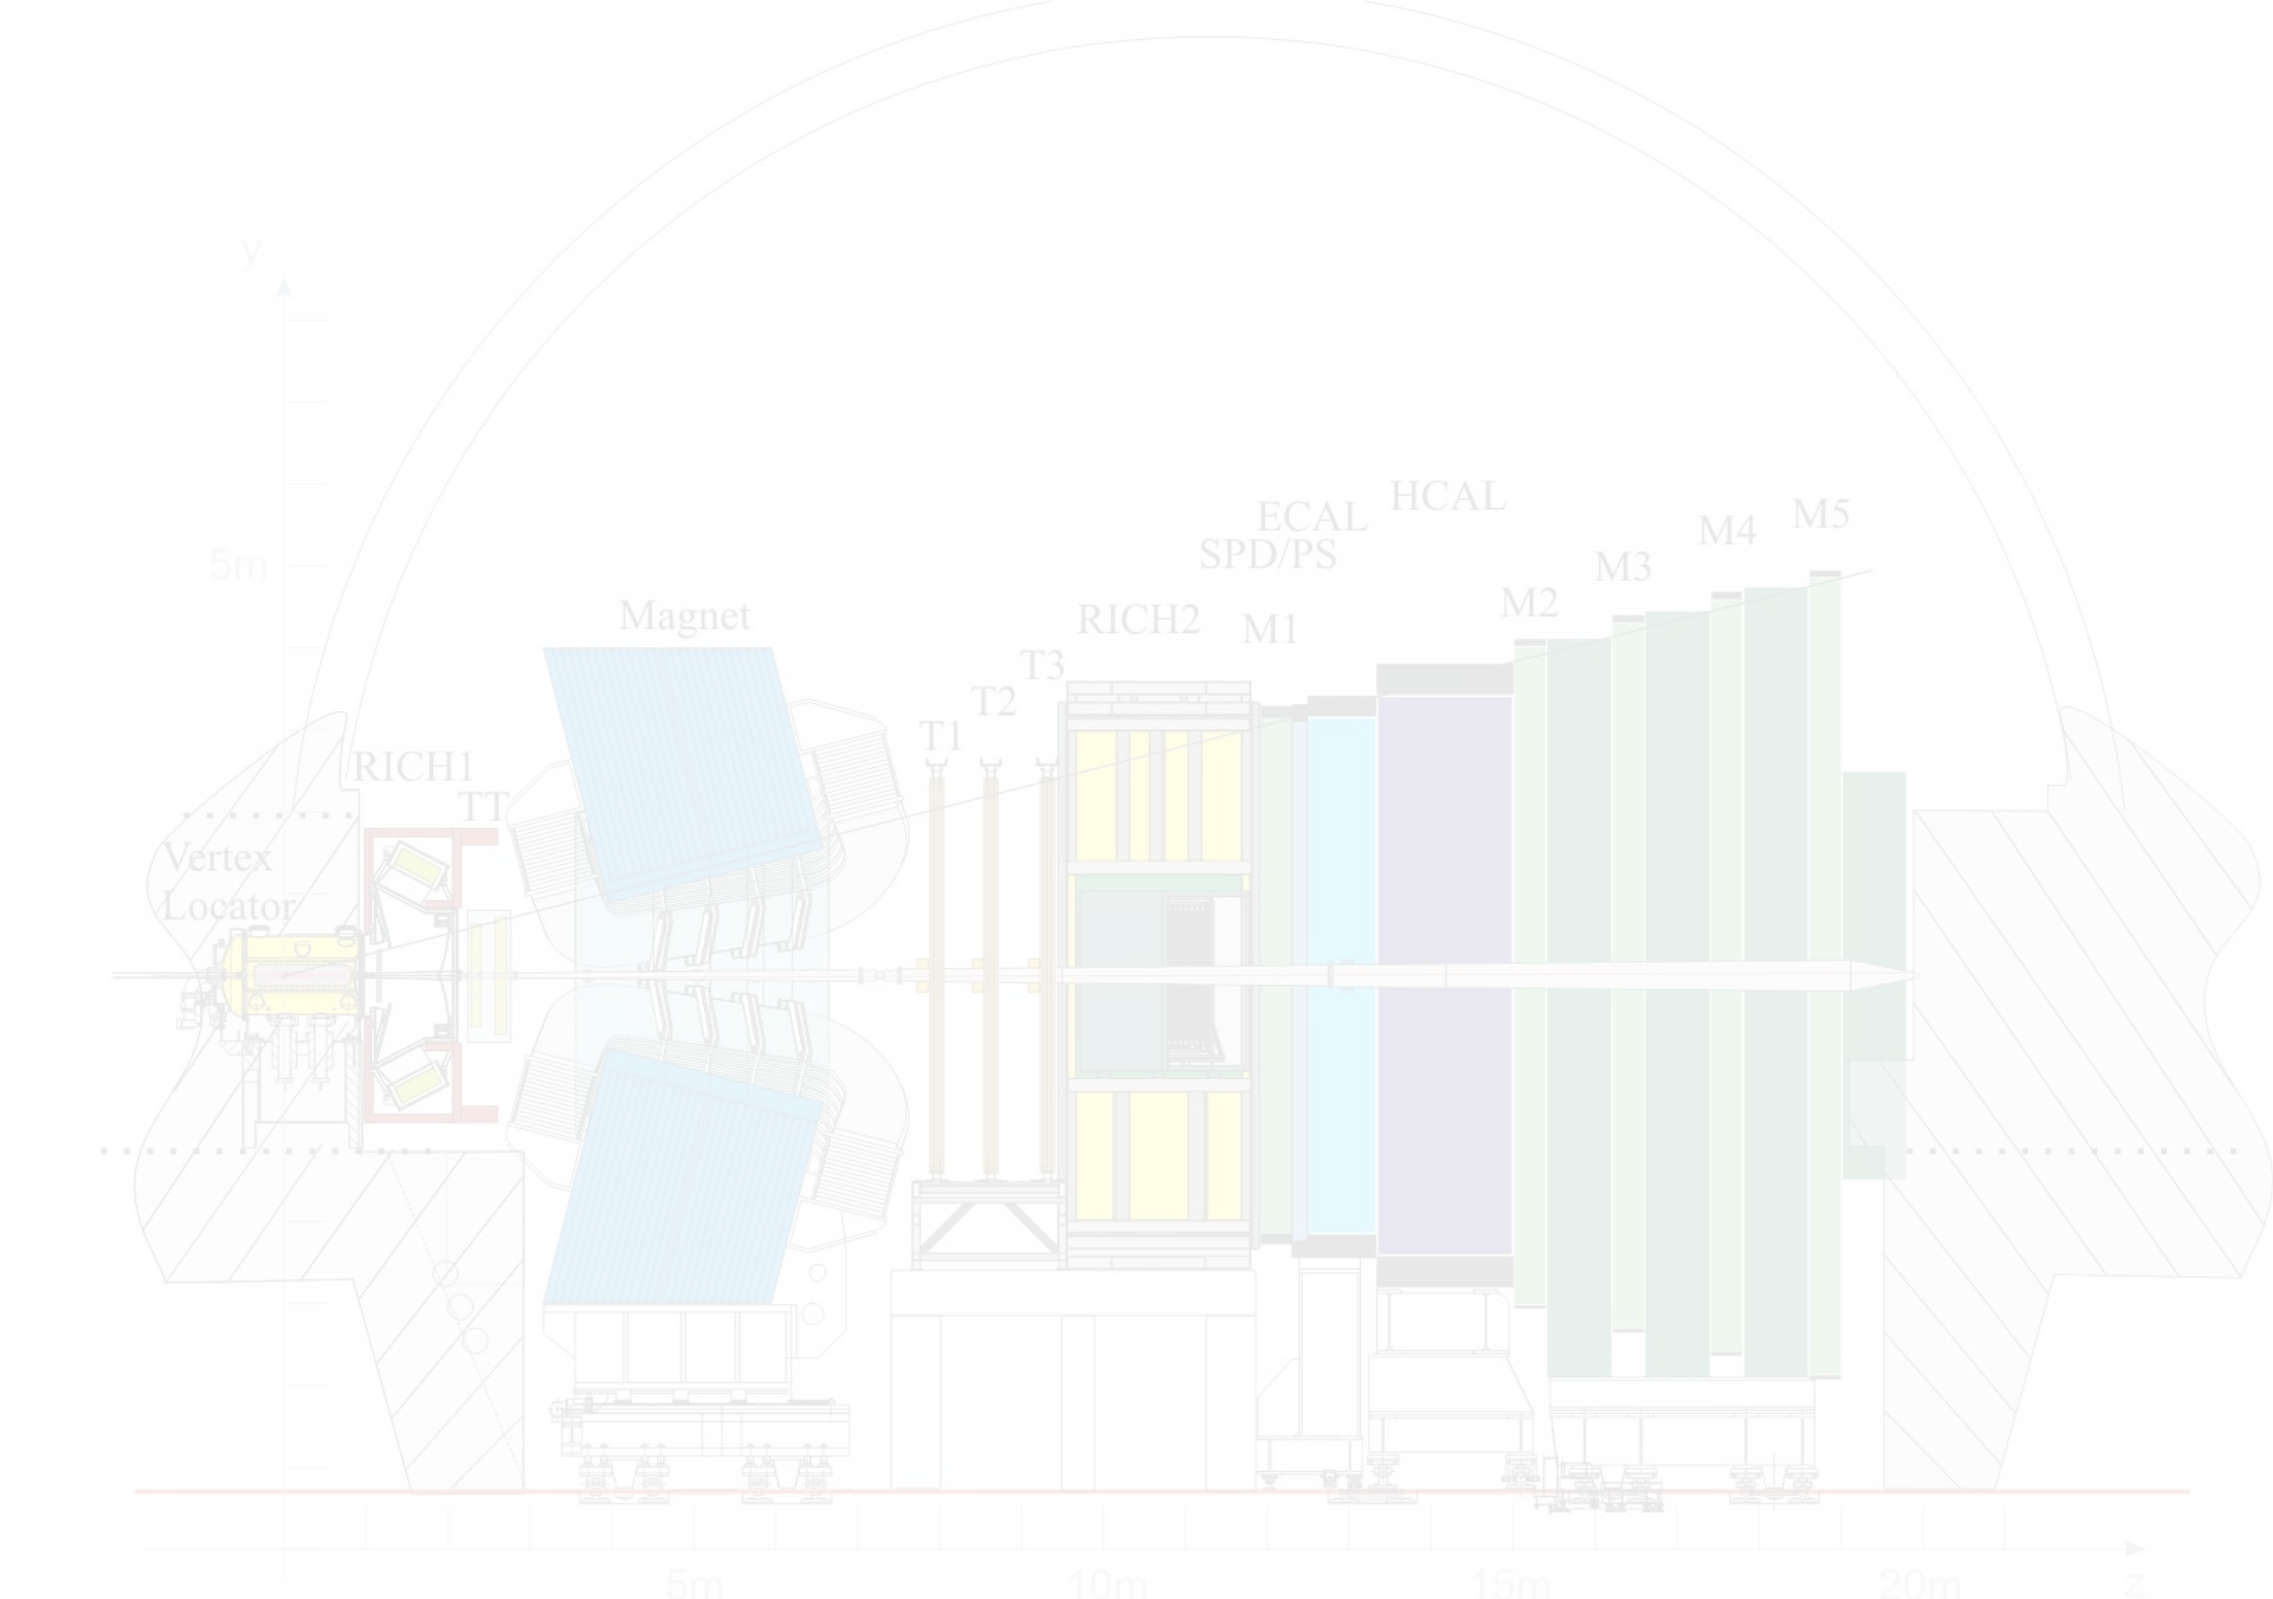
\includegraphics[width=\paperwidth]{gene-2008-002_01_t2}}

\begin{frame}
\frametitle{PhD.: Physics content}
Title: Calibration of the flavour tagging algorithm of the LHCb experiment by
the measurement of $\sin(2\phi_1)$\\
~\\
\begin{itemize}
  \item Selection of control channels: $\PBu\to\PJpsi\PKplus$ and
  $\PBd\to\PJpsi\PKstar^0$
  \item Measurement of the mistag fraction using $\PBd$ mixing property
  \item Measurement of $\sin(2\phi_1)$ in $\PBd\to\PJpsi\PKshort$ using
  previously measured mistag rate, systematics' studies
\end{itemize}
\begin{columns}[t]
\begin{column}[T]{4cm}
\begin{block}{$\PBu\to\PJpsi\PKplus$}
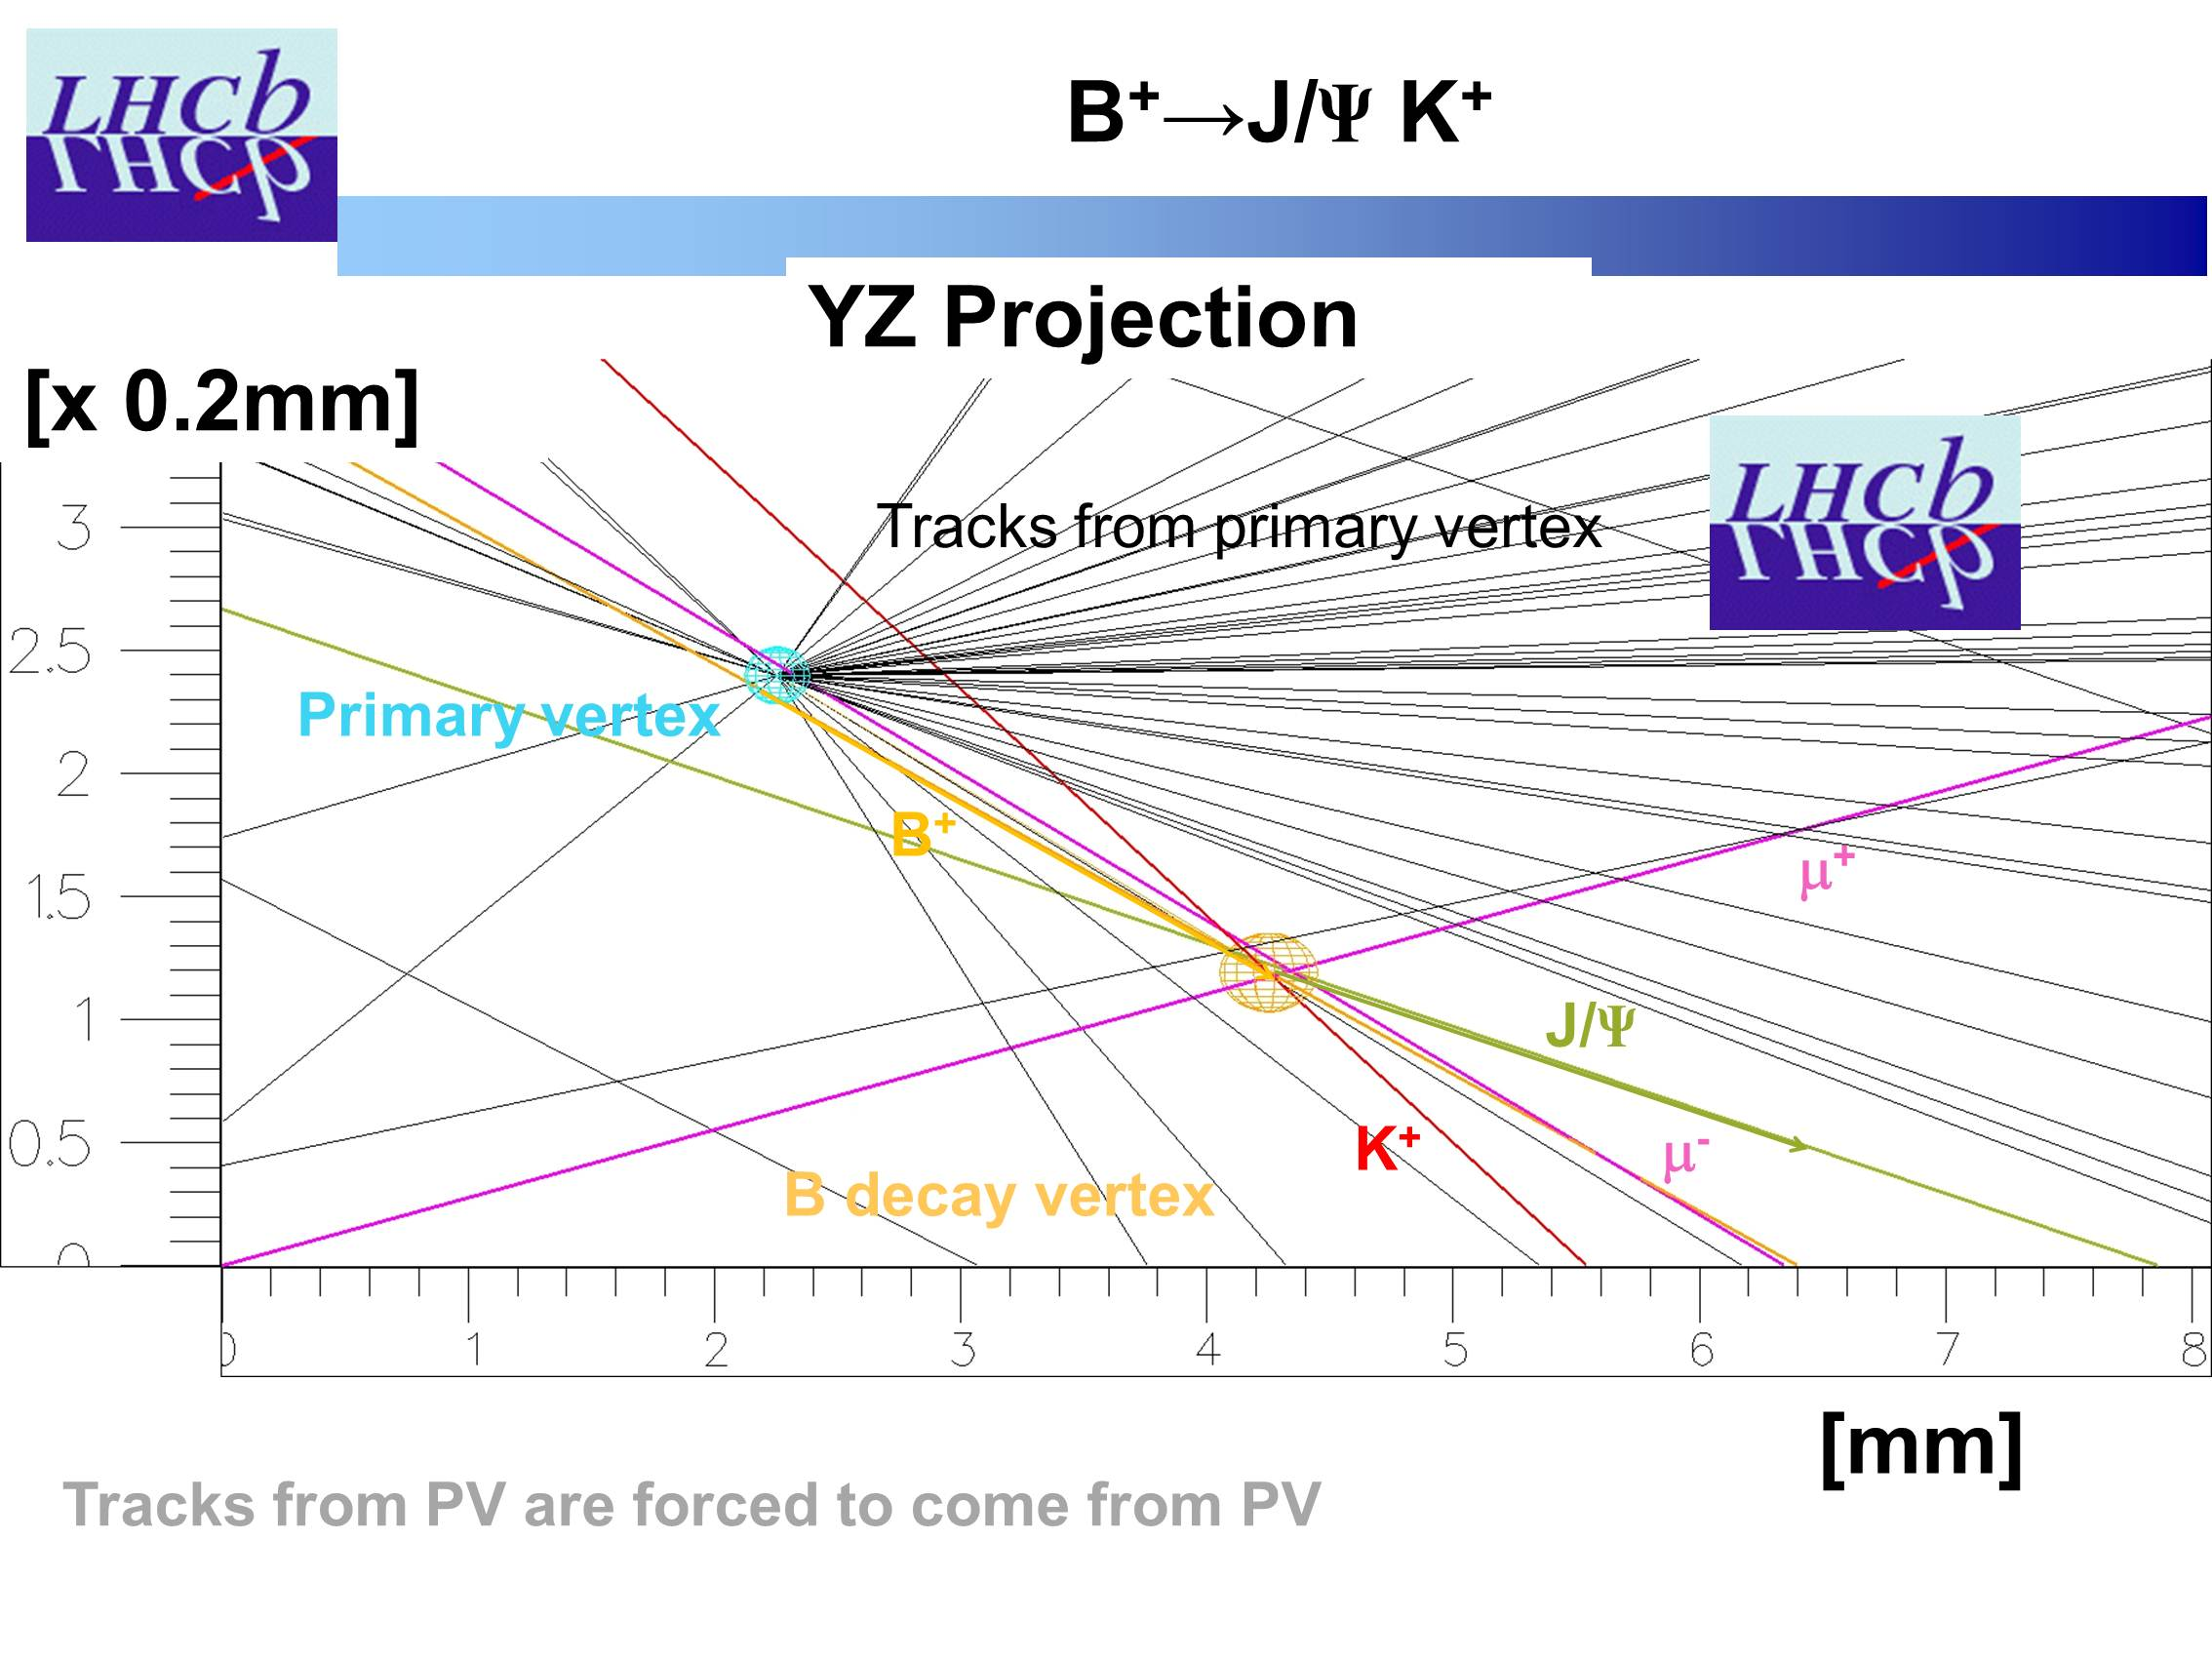
\includegraphics[width=4cm]{s7}
\end{block}
\end{column}
\begin{column}[T]{4cm}
\begin{block}{Mistag fraction}
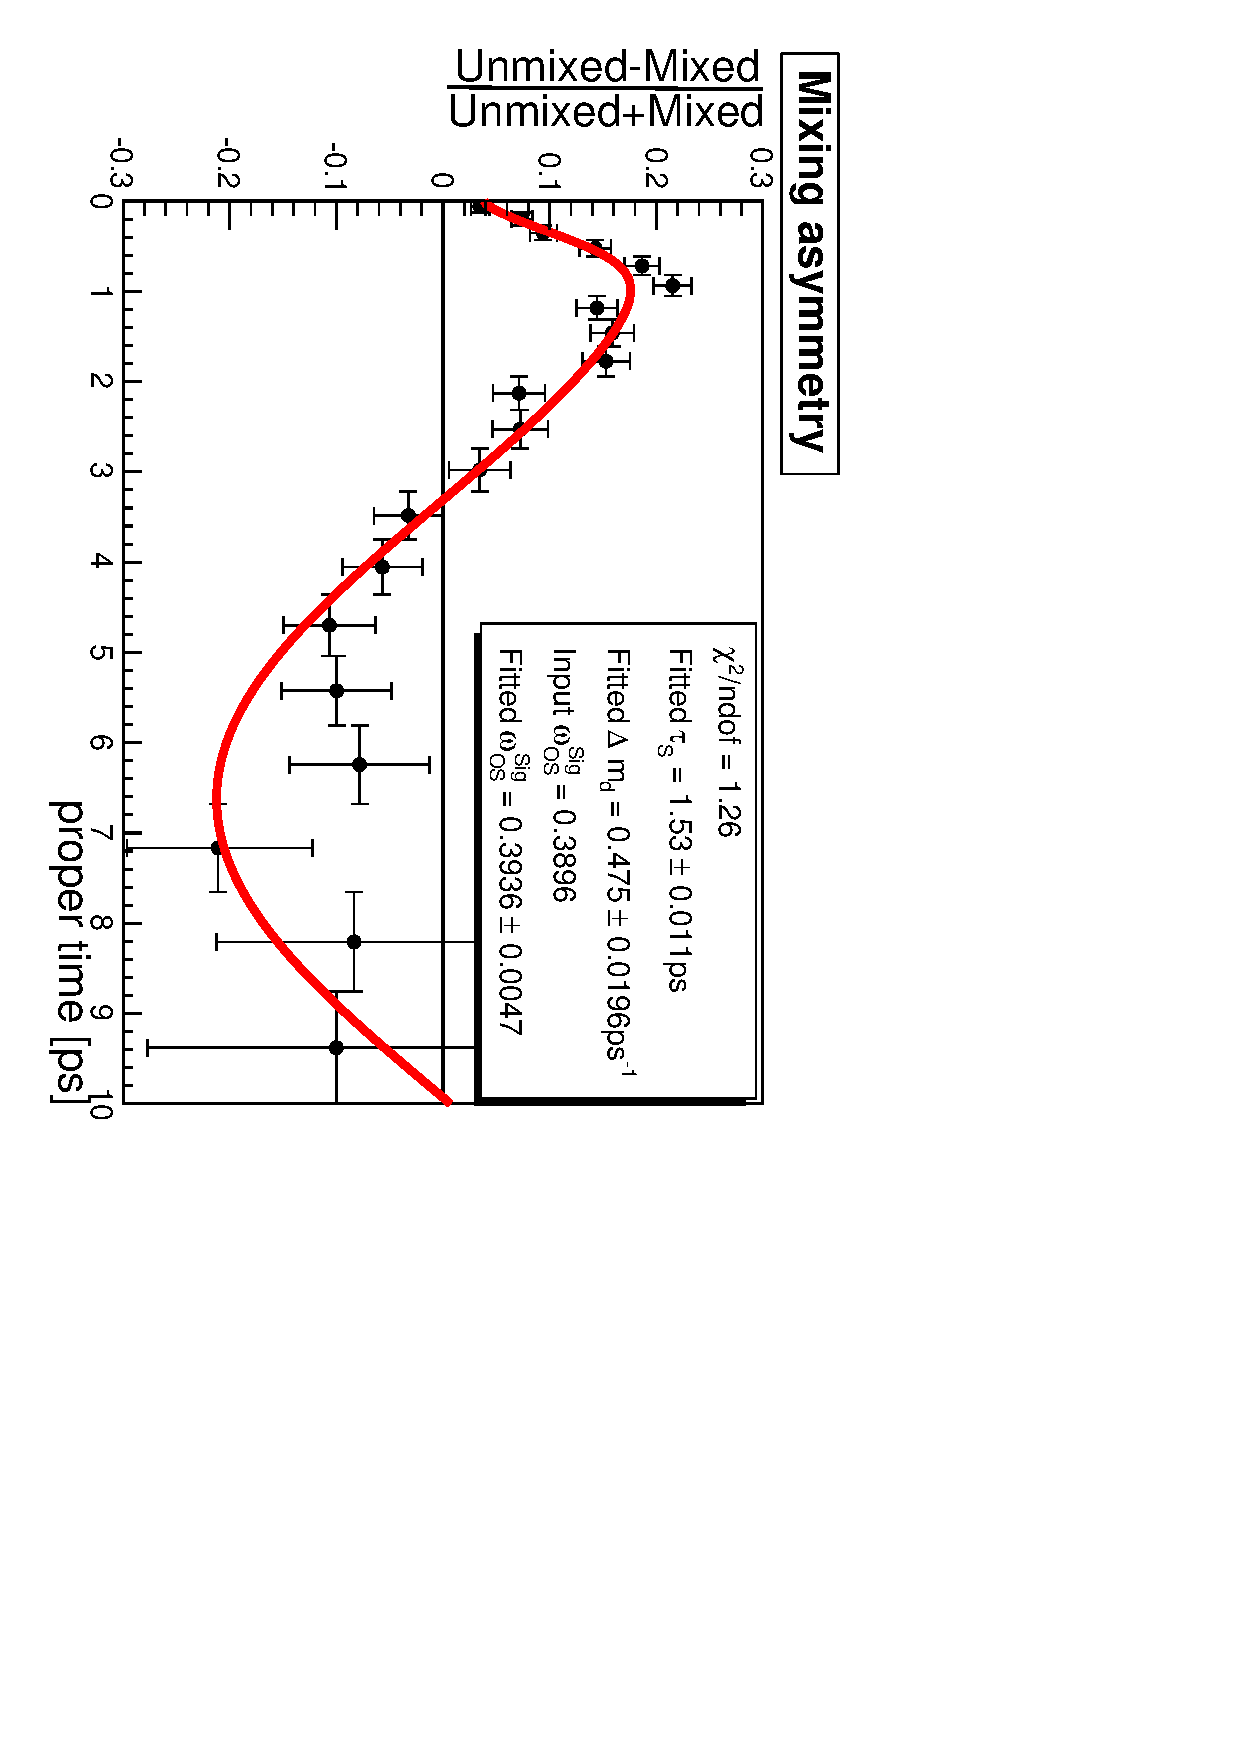
\includegraphics[angle=90,width=4cm]{CombinedAsymFit}
\end{block}
\end{column}
\begin{column}[T]{4cm}
\begin{block}{$\sin(2\phi_1)$}
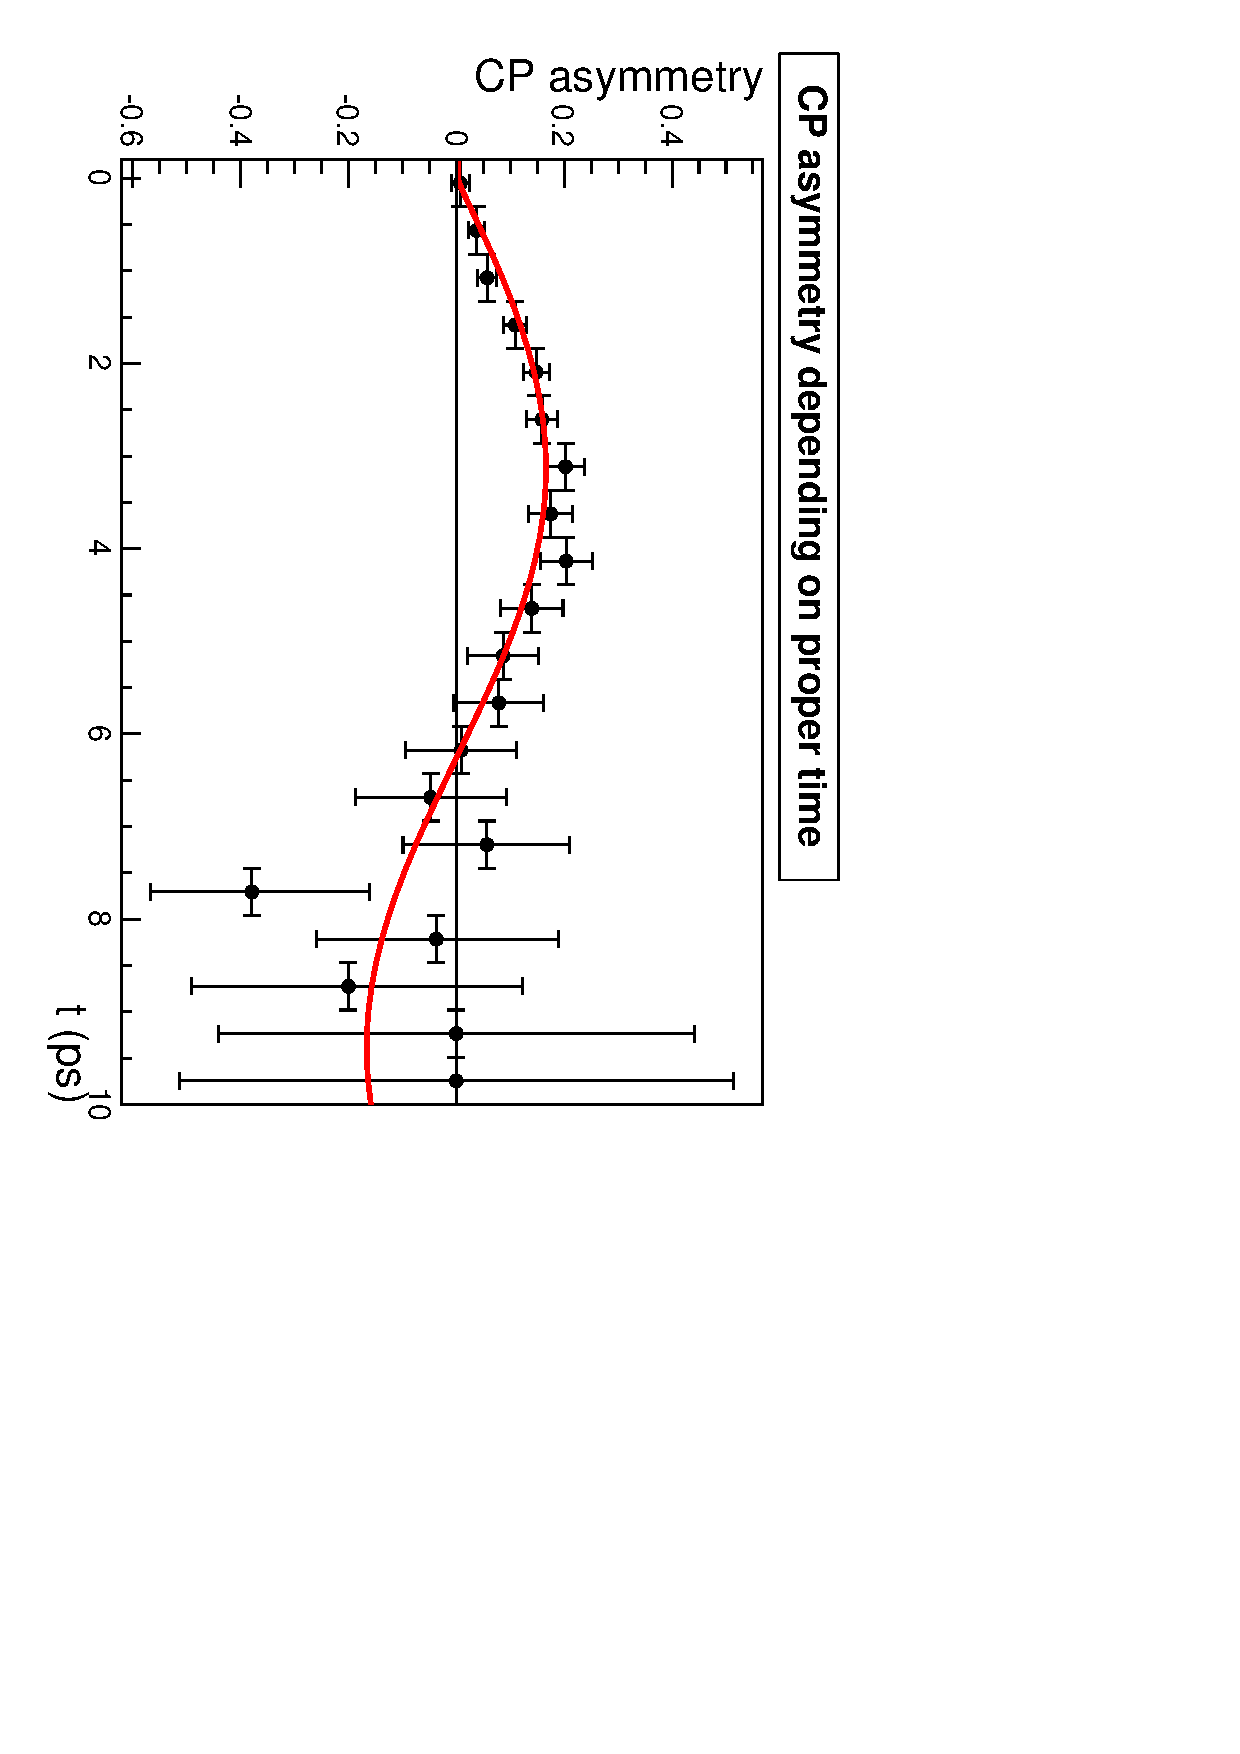
\includegraphics[angle=90,width=4cm]{AsymCPDC06AverageOmega}
\end{block}
\end{column}
\end{columns}
\end{frame}

% \begin{frame}
% \frametitle{PhD.: Using DIRAC in LHCb}
% Several {\color{blue}millions of events} to analyse + {\color{blue}thousands of
% toy MC studies}: used DIRAC a lot.
% \begin{center}
% 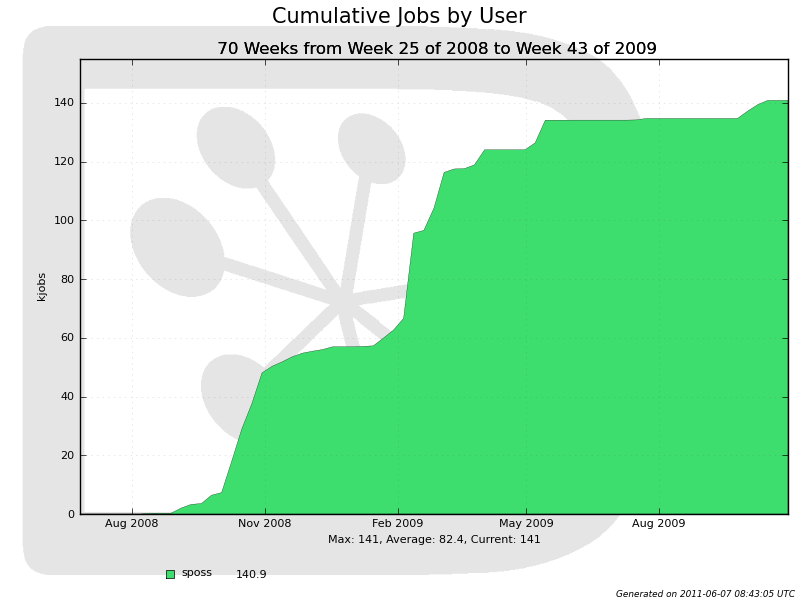
\includegraphics[width=8cm]{sposs_user}
% \end{center}
% I wanted to \alert{be involved in the development of this tool}.
% \end{frame}
}


{
\usebackgroundtemplate{
\includegraphics[width=10cm]{cern_logo_white}}

\part{Fellowship, 2010-now}
\begin{frame}
\partpage
\end{frame}
}
\begin{frame}
\frametitle{The project}
\begin{itemize}
  \item Applied for \alert{fellowship at CERN}, emphasis on {\color{blue}DIRAC
  in LHCb}: distributed analysis
  \item Contacted by L. Linssen ({\color{blue}Linear Collider Detectors group}) to develop a
  \alert{DIRAC client} for the ILC Virtual Organization (ILC and CLIC):\\ 
  \begin{itemize}  
    \item Aim was \alert{mass production of Monte Carlo data} for the CLIC
    Conceptual Design Report (CDR): {\color{blue}benchmark of 2 detector
    concepts}
    \item Document {\color{blue} finished in 2011}: needed fast solution
    \item DIRAC was proven by LHCb to be \alert{efficient}
    \item Should be usable by Linear Collider community
    %\item DIRAC team wanted to show it could be used outside LHCb
  \end{itemize}
\end{itemize}
\end{frame}

\begin{frame}
\frametitle{Linear Collider detectors}
\begin{columns}
\begin{column}{6cm}
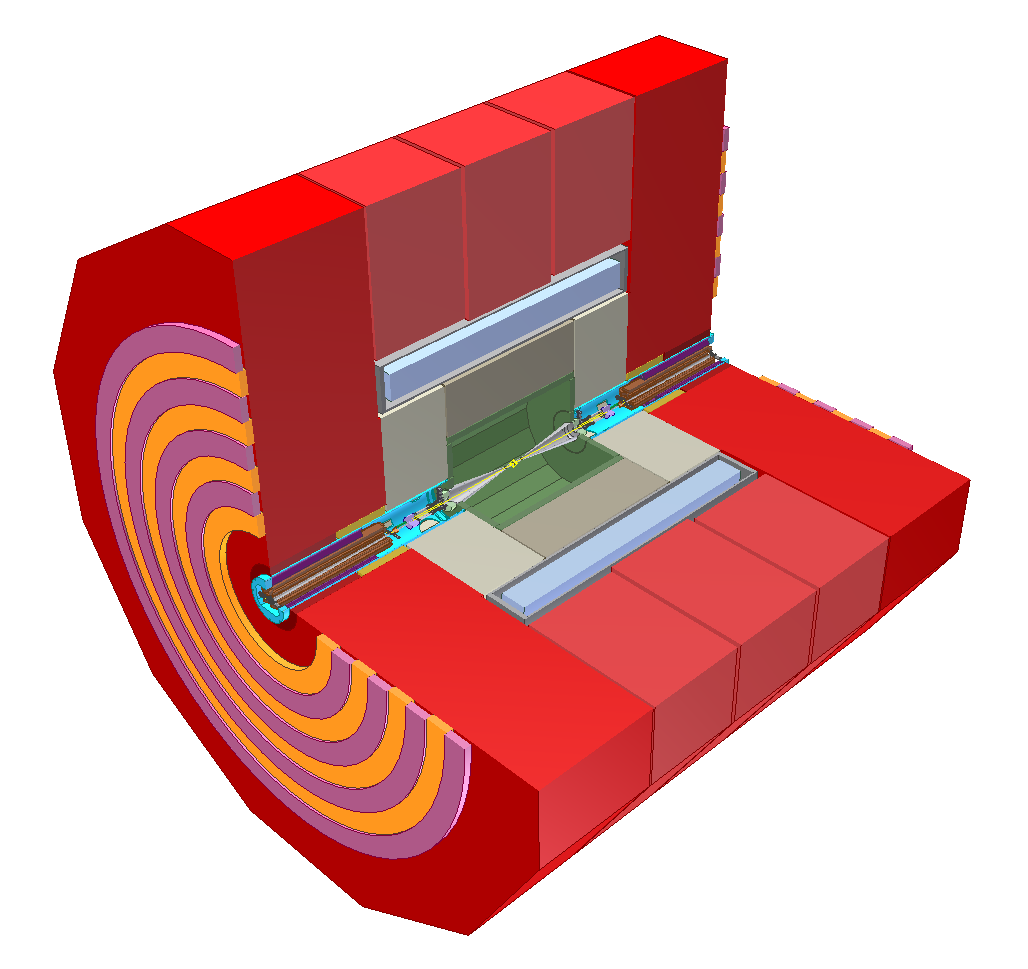
\includegraphics[width=6cm]{Detectors.png}
\end{column}
\begin{column}{5cm}
ILC and CLIC are future Linear Colliders\\
~\\
Detectors' design similar to CMS\\
~\\
Main difference between concepts: {\color{blue}the tracking system}
\begin{itemize}
  \item ILD uses a TPC
  \item SiD uses silicon layers
\end{itemize}
\end{column}
\end{columns}
\end{frame}

{
\usebackgroundtemplate{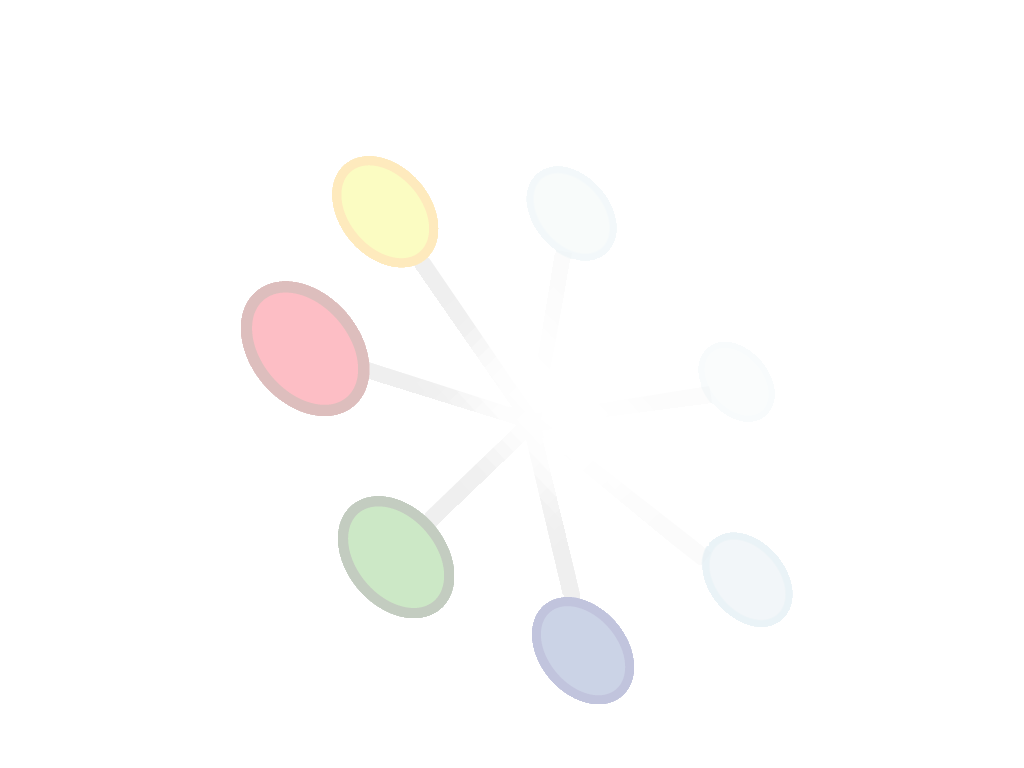
\includegraphics[width=\paperwidth]{DiracVisual}} 
 
\begin{frame}
\frametitle{The ILCDIRAC client}
ILCDIRAC: DIRAC client dedicated to the {\color{blue}linear collider
community}:
\begin{itemize}
  \item ILC and CLIC share the same virtual organisation and same softwares
  \item \alert{Convenient interface} to handle ILC applications: 12
different types with different user interfaces
\item Written in {\color{blue}PYTHON} to follow DIRAC framework
\item \alert{Documentation} to be usable by many others
\item Now \alert{adopted by the ILC SID community} for their Detailed Baseline
  Design document mass production
\end{itemize}
\end{frame}

\begin{frame}
  \frametitle{Usage}
ILCDIRAC client was used for:
\begin{itemize}
  \item Mass Monte Carlo \alert{production}: CLIC CDR and SID DBD\\~\\
  \item User jobs: \alert{analysis} for ILC and CLIC\\~\\
  \item \alert{Data management: File Catalog} was essential for those activities\\~\\
\end{itemize}
~\\
More than {\color{blue}6 million jobs processed in 2.5 year}\\
~\\
Users not only at CERN, but also LAL (FR.), MPI (DE.), VINCA (R.S.),
SLAC (U.S.A), etc.
\end{frame}

\begin{frame}
\frametitle{My current activities}
ILCDIRAC management:\\
\begin{itemize}
  \item Development of \alert{new features}~\\ ~\\
  \item Realisation of \alert{documentation}: tutorial slides, online code
  documentation~\\ ~\\
  \item \alert{Monitoring} of system status: VOBOX and grid resources~\\ ~\\
  \item {\color{blue}Installation and setup} of services
\end{itemize}
\end{frame}
}

{
\usebackgroundtemplate{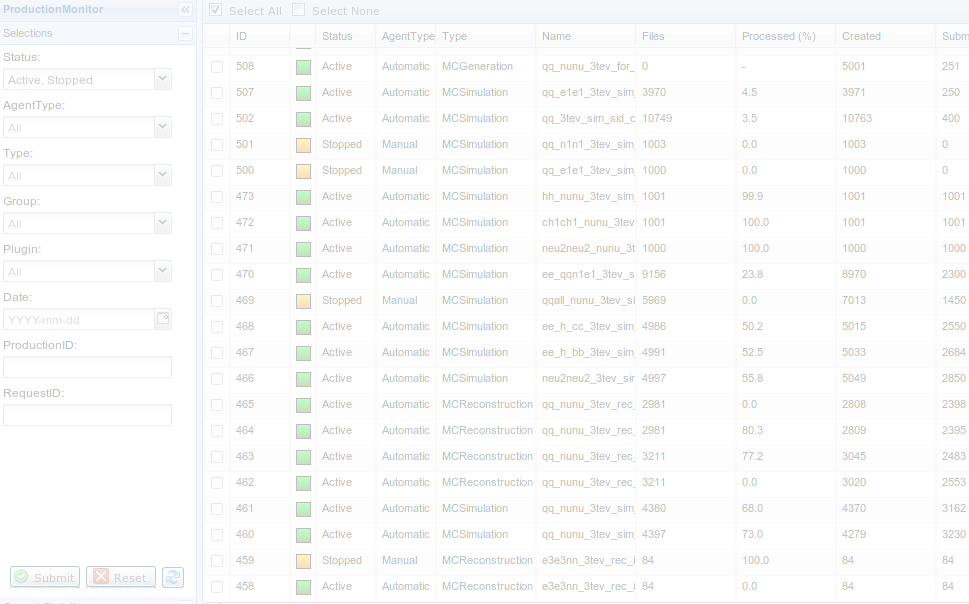
\includegraphics[width=\paperwidth]{prod_mon2}}

\begin{frame} 
\frametitle{My current activities (Cont'd)}
Mass Production:\\
\begin{itemize}
  \item \alert{Production manager}: definition of new productions, monitor
  statuses, produce statistics~\\ ~\\
  \item {\color{blue}Data manager}: make sure the data is where it's supposed to
  be, replicate when needed, check availability of resources
\end{itemize}
\end{frame}
}
% {
% \usebackgroundtemplate{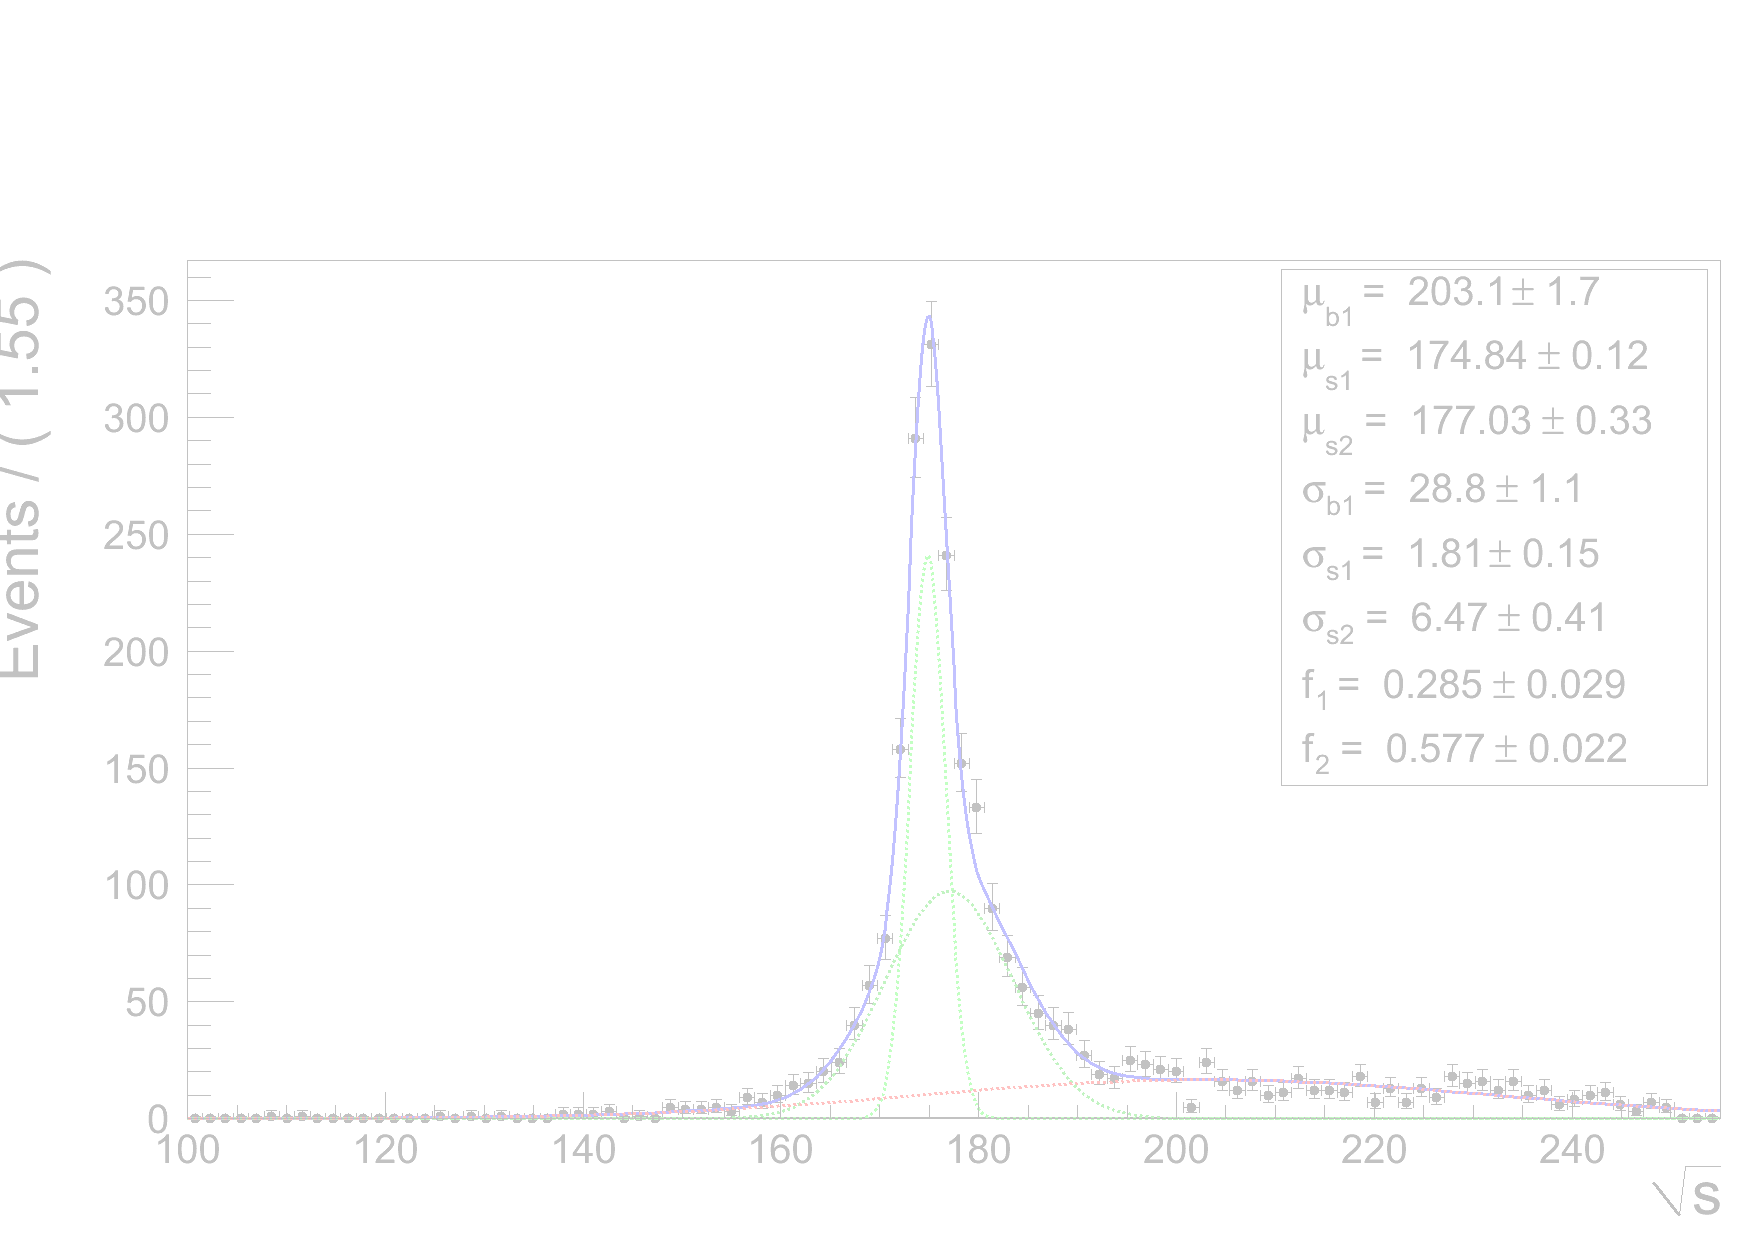
\includegraphics[width=\paperwidth]{tt-mass2}} 

% \begin{frame}
% \frametitle{Current activities (Cont'd)}
% Convener of the $\Ptop\APtop$ at $\sqrt{s}=$500~GeV analysis:\\
% \begin{itemize}
%   \item One of the 6 benchmark channels for the CLIC detectors~\\ ~\\
%   \item Interesting as a comparison point with ILC detectors
% \end{itemize}
% \end{frame}
%  }
%  {
% \usebackgroundtemplate{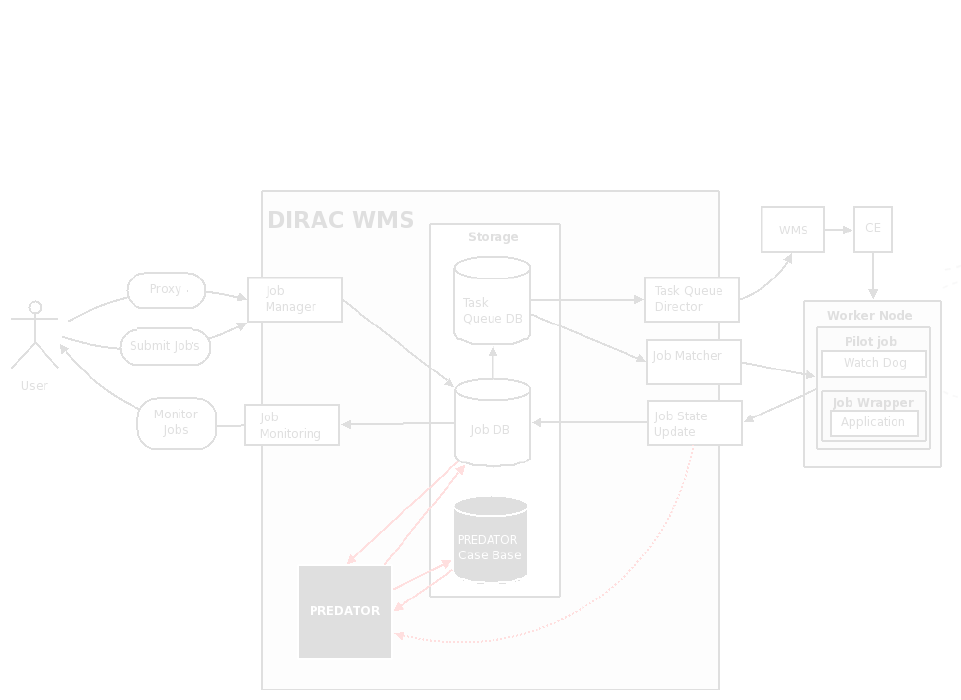
\includegraphics[width=\paperwidth]{predator}} 
 
%  \begin{frame}
%  \frametitle{Student supervision}
%  P. Majewski (Master student): 
%  \begin{itemize}
%    \item Initial developments of ILCDIRAC
%  \end{itemize}
%  ~\\
%  C.~B.~Lam (Bachelor student):
% \begin{itemize}
%   \item Quality control of Production Data
%   \item Jet energy resolution effects on top quark mass measurements
%   \item Review of ILCDIRAC user interface
% \end{itemize}
% ~\\
% E. Hidle (Master student):
% \begin{itemize}
%   \item GRID job running time predictions, using Case Based Reasoning in the
%   ILCDIRAC context
% \end{itemize}
%  \end{frame}
% }

{
\usebackgroundtemplate{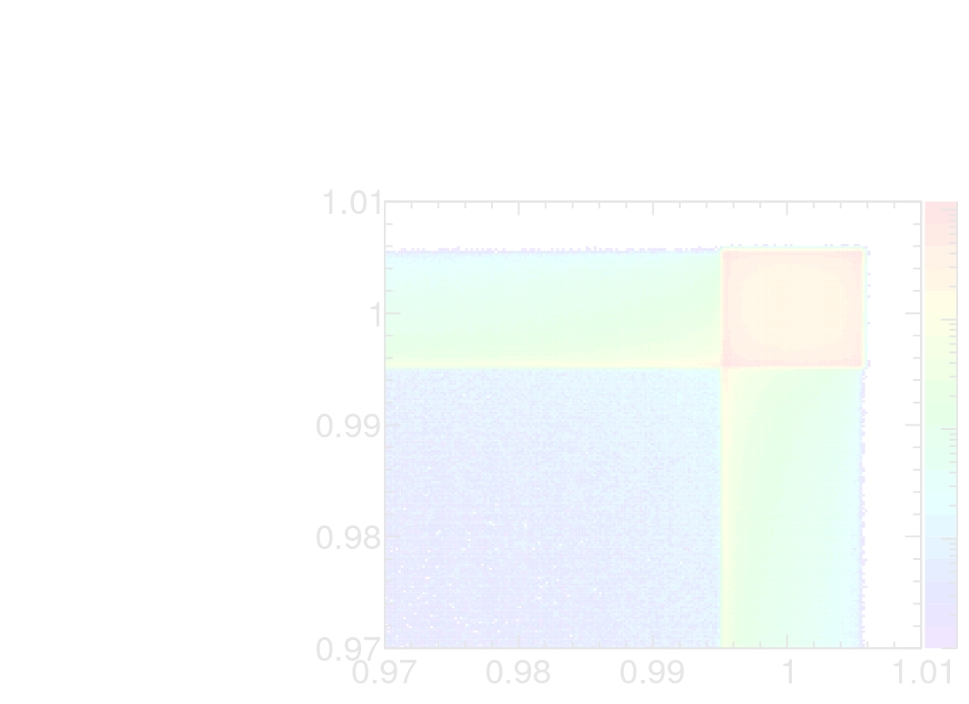
\includegraphics[width=\paperwidth]{LumiSpectrum}}
  \begin{frame}
    \frametitle{My current activities (Cont'd)}
    Measurement of the \alert{luminosity spectrum} (at CLIC 3TeV):
    \begin{itemize}
      \item Needed for {\color{blue}precise cross section} measurements\\ ~\\
      \item Understand \alert{beam-beam interactions}~\\ ~\\
      \item Implement models using \alert{Object Oriented principles} (C++)~\\ ~\\
      \item Provide spectra to users accounting for statistical and
        systematic errors
    \end{itemize}
  \end{frame}
}
\part{Contributions to Belle II}
{
\usebackgroundtemplate{
\includegraphics[width=\paperwidth]{belle2-logo_transp}}
\begin{frame}
\partpage
\end{frame}
\begin{frame}
  \frametitle{Computing}
Development:
\begin{itemize}
\item DIRAC mass {\color{blue}production system}
\item Data Catalog: \alert{DIRAC File Catalog}
\item Improve \alert{user interface}
\item Data management: {\color{blue}popularity}
\end{itemize}
~\\
Operations:
\begin{itemize}
\item Interface with Computing Elements: Amazon EC2, GRID (PNNL)
\item Service monitoring, machine management
\item Data replication, production management
\item Training
\end{itemize}
\end{frame}

\begin{frame}
  \frametitle{Physics}
Data analysis:
  \begin{itemize}
  \item Flavour tagging optimization and calibration
  \item Background rejection
  \item Luminosity spectrum measurement
  \item $\PB\to \tau \nu$
  \end{itemize}
\end{frame}
}
\part{Future: ILC}
\begin{frame}
\partpage
\end{frame}
\begin{frame}
  \frametitle{Long term work: ILC}
 ILC will need computing infrastructures:
 \begin{itemize}
  \item High event rate
  \item High event density
  \item International collaboration: data distribution
 \end{itemize}
Already familiar with:
\begin{itemize}
\item Detector frameworks
\item Physics conditions
\item Software environment
\end{itemize}
\end{frame}
 % \begin{frame}
 %   \vskip 5cm 
 %   \centering
 %   %toto
 %   % \begin{CJK}{utf8}{min}
 %   \begin{CJK}{UTF8}{min}
 %     ���꤬�Ȥ�
 %   \end{CJK}
 %\end{frame}
 \part{Summary in relation to offered position}
 \begin{frame}
 \partpage
 \end{frame}
 \begin{frame}
 \frametitle{Summary} 
 \begin{itemize}
 \item \alert{Computing infrastructure} development
   and operation:
   \begin{itemize}
   \item {\color{blue}DIRAC for Belle 2}
   \item {\color{blue}Production} activities
   \item {\color{blue}Simulation and Reconstruction} software frameworks
   \end{itemize}
   ~\\
 \item \alert{Data} taking and analysis:
   \begin{itemize}
   \item {\color{blue}CP violation} still has a lot to tell
   \item {\color{blue}Rare decays} can provide hints on New Physics
   \item Very exciting subject! 
   \end{itemize}
   ~\\
 \item The future: \alert{ILC}
 \end{itemize}
%~\\
%\hspace{0.6\textwidth} \scriptsize{Japan is a fascinating country!}  
 \end{frame}

\appendix
\begin{frame}
  \frametitle{Backups}
\end{frame}
{
\usebackgroundtemplate{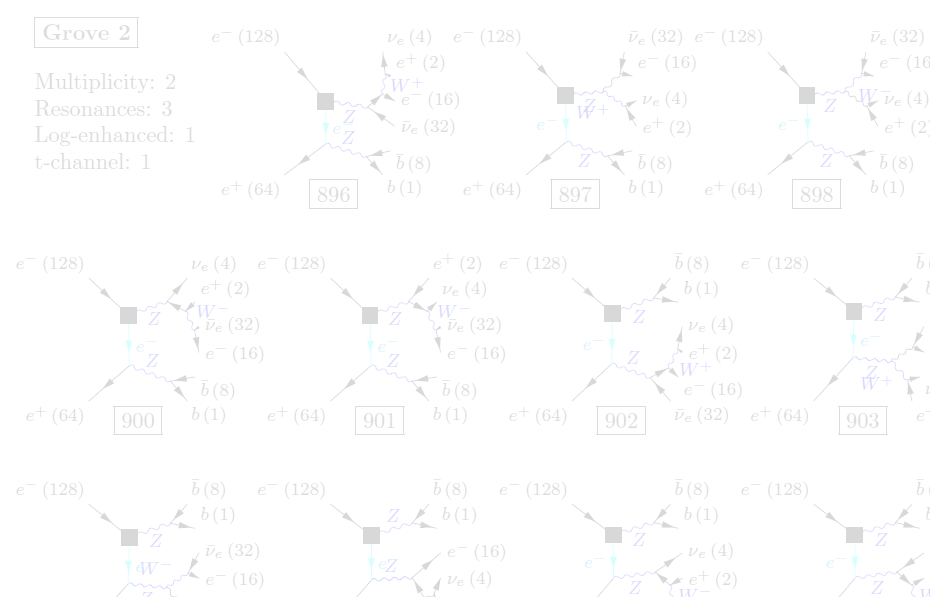
\includegraphics[width=\paperwidth]{process_ex_1}}

\begin{frame}
\frametitle{Other activities}
Physics generation:\\
\begin{itemize}
  \item Setup framework for {\color{blue} convenient physics generation}: 2
  generators, WHIZARD and PYTHIA~\\ ~\\
  \item Implement channels in the 2 generators used, perform tests~\\ ~\\
  \item \alert{Interface to ILCDIRAC}
\end{itemize}
CERN representative of the working group dedicated to {\color{blue}common
generator tools for the Linear Colliders}.
\end{frame}
}

\end{document}
% Local Variables:
% TeX-PDF-mode: t
% coding: euc-japan
% End:
